% C.25 △ABC 中位线 DE
\documentclass[tikz,border=4pt]{standalone}
\usepackage{ctex}
\usepackage{amsmath}
\usetikzlibrary{calc, arrows.meta}
\begin{document}
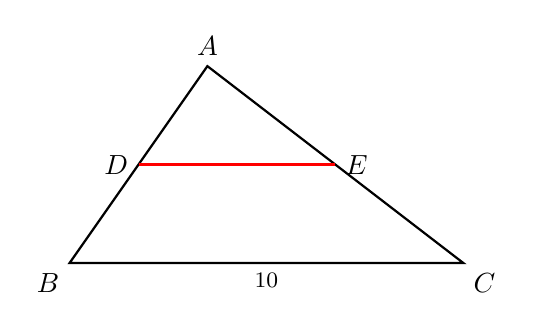
\begin{tikzpicture}[scale=0.5, thick]
  \coordinate (B) at (0,0);
  \coordinate (C) at (10,0);
  \coordinate (A) at (3.5,5);
  \coordinate (D) at ($(A)!0.5!(B)$);
  \coordinate (E) at ($(A)!0.5!(C)$);
  \draw (A) -- (B) -- (C) -- cycle;
  \draw[red] (D) -- (E);
  \node[above] at (A) {$A$};
  \node[below left] at (B) {$B$};
  \node[below right] at (C) {$C$};
  \node[left] at (D) {$D$};
  \node[right] at (E) {$E$};
  \node[font=\footnotesize, below] at (5,0) {$10$};
\end{tikzpicture}
\end{document}
